\chapter{Cerca completa}

\key{Cerca completa}
és un mètode general que es pot fer servir
per a resoldre gairebé qualsevol problema algorísmic.
La idea és generar totes les possibles
solucions del problema amb força bruta
i, a continuació, seleccionar la millor solució, o comptar
el nombre de solucions, segons el problema.

La cerca completa és una bona tècnica
si hi ha prou temps per a generar totes les solucions,
ja que la cerca sol ser fàcil d'implementar
i sempre dóna la resposta correcta.
Si la cerca completa és massa lenta haurem
de fer servir altres tècniques, com els algorismes \emph{greedy}
o la programació dinàmica.

\section{Generar subconjunts}

\index{subconjunt}

Considerem el problema de generar
tots els subconjunts d'un conjunt de $n$ elements.
Per exemple, els subconjunts de $\{0,1,2\}$ són
$\emptyset$, $\{0\}$, $\{1\}$, $\{2\}$, $\{0,1\}$,
$\{0,2\}$, $\{1,2\}$ i $\{0,1,2\}$.
Hi ha dos mètodes comuns per a generar subconjunts:
fer una cerca recursiva
o aprofitar la representació binària dels nombres enters.

\subsubsection{Mètode 1}

La recursivitat és una manera elegant de passar per
tots els subconjunts d'un conjunt.
La següent funció \texttt{search}
genera els subconjunts de
$\{0,1,\ldots,n-1\}$.
La funció manté un vector global \texttt{v}
que anirà contenint els elements de cada subconjunt.
La cerca comença quan es crida la funció
amb el paràmetre 0.

\begin{lstlisting}
vector<int> v;

void cerca(int k) {
    if (k == n) {
        // tracta el subconjunt v;
    } altrament {
        cerca(k+1);
        v.push_back(k);
        cerca(k+1);
        v.pop_back();
    }
}
\end{lstlisting}

Quan la funció \texttt{cerca}
es crida amb el paràmetre $k$,
aquesta decideix si inclou o no l'element $k$ al subconjunt
i, en ambdós casos,
es crida recursivament a ella mateixa amb paràmetre $k+1$.
Tanmateix, si $k=n$, la funció s'adona
que ha processat tots els elements
i, per tant, s'ha generat un nou subconjunt $v$.

L'arbre següent il·lustra les crides de funció quan $n=3$.
Sempre podem triar la branca esquerra
($k$ no s'inclou al subconjunt) o la branca dreta
($k$ s'inclou al subconjunt).

\begin{center}
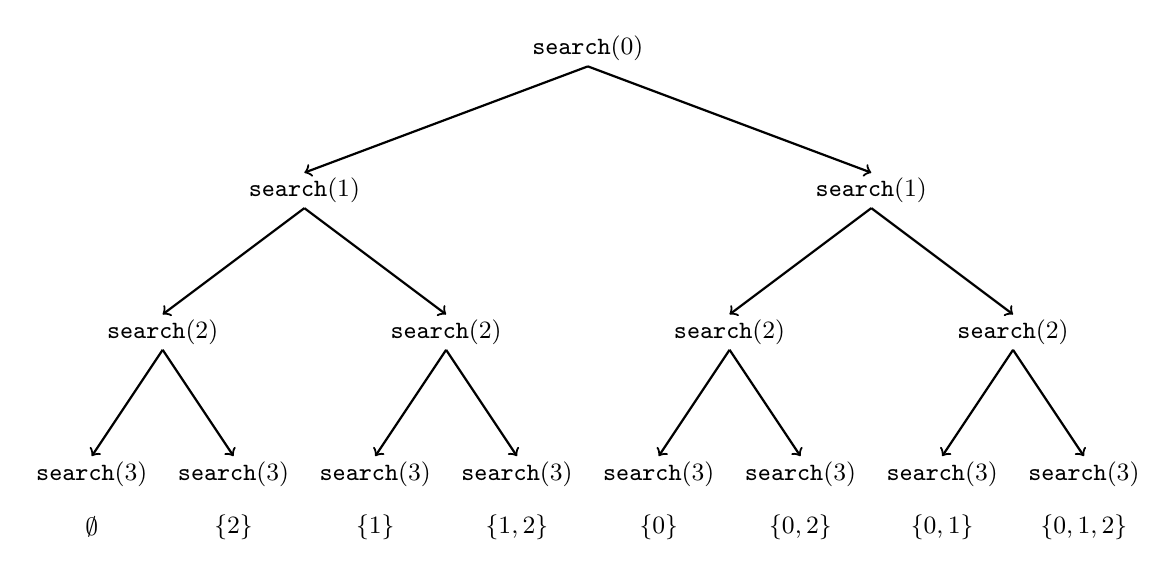
\begin{tikzpicture}[scale=.45]
  \begin{scope}
    \small
    \node at (0,0) {$\texttt{search}(0)$};

    \node at (-8,-4) {$\texttt{search}(1)$};
    \node at (8,-4) {$\texttt{search}(1)$};

    \path[draw,thick,->] (0,0-0.5) -- (-8,-4+0.5);
    \path[draw,thick,->] (0,0-0.5) -- (8,-4+0.5);

    \node at (-12,-8) {$\texttt{search}(2)$};
    \node at (-4,-8) {$\texttt{search}(2)$};
    \node at (4,-8) {$\texttt{search}(2)$};
    \node at (12,-8) {$\texttt{search}(2)$};

    \path[draw,thick,->] (-8,-4-0.5) -- (-12,-8+0.5);
    \path[draw,thick,->] (-8,-4-0.5) -- (-4,-8+0.5);
    \path[draw,thick,->] (8,-4-0.5) -- (4,-8+0.5);
    \path[draw,thick,->] (8,-4-0.5) -- (12,-8+0.5);

    \node at (-14,-12) {$\texttt{search}(3)$};
    \node at (-10,-12) {$\texttt{search}(3)$};
    \node at (-6,-12) {$\texttt{search}(3)$};
    \node at (-2,-12) {$\texttt{search}(3)$};
    \node at (2,-12) {$\texttt{search}(3)$};
    \node at (6,-12) {$\texttt{search}(3)$};
    \node at (10,-12) {$\texttt{search}(3)$};
    \node at (14,-12) {$\texttt{search}(3)$};

    \node at (-14,-13.5) {$\emptyset$};
    \node at (-10,-13.5) {$\{2\}$};
    \node at (-6,-13.5) {$\{1\}$};
    \node at (-2,-13.5) {$\{1,2\}$};
    \node at (2,-13.5) {$\{0\}$};
    \node at (6,-13.5) {$\{0,2\}$};
    \node at (10,-13.5) {$\{0,1\}$};
    \node at (14,-13.5) {$\{0,1,2\}$};


    \path[draw,thick,->] (-12,-8-0.5) -- (-14,-12+0.5);
    \path[draw,thick,->] (-12,-8-0.5) -- (-10,-12+0.5);
    \path[draw,thick,->] (-4,-8-0.5) -- (-6,-12+0.5);
    \path[draw,thick,->] (-4,-8-0.5) -- (-2,-12+0.5);
    \path[draw,thick,->] (4,-8-0.5) -- (2,-12+0.5);
    \path[draw,thick,->] (4,-8-0.5) -- (6,-12+0.5);
    \path[draw,thick,->] (12,-8-0.5) -- (10,-12+0.5);
    \path[draw,thick,->] (12,-8-0.5) -- (14,-12+0.5);
\end{scope}
\end{tikzpicture}
\end{center}

\subsubsection{Mètode 2}

Una altra manera de generar subconjunts es fer servir
la representació en binari dels nombres enters.
Cada subconjunt d'un conjunt de $n$ elements
es pot representar com una seqüència de $n$ bits,
que correspon a un nombre enter entre $0 \ldots 2^n-1$.
Els uns en la seqüència de bits indiquen
quins elements formen part del subconjunt.

La convenció habitual és que
l'últim bit correspon a l'element 0,
el penúltim bit és l'element 1,
etcètera.
Per exemple, la representació binària de 25
és 11001, que correspon al subconjunt $\{0,3,4\}$.

El codi següent\footnote{N. del T.: La notació \texttt{1<<n} és l'operador \emph{shift}, i indica que el nombre 1 es desplaça $n$
posicions a l'esquerra, és a dir, $2^n$}
tracta tots els subconjunts d'un conjunt de $n$ elements

\begin{lstlisting}
for (int b = 0; b < (1<<n); b++) {
    // tracta el subconjunt b
}
\end{lstlisting}

El codi següent mostra com trobar el subconjunt que conté
els elements corresponents a una seqüència de bits.
Quan tractem cada subconjunt $b$, el codi construeix el vector
$v$ amb els elements del subconjunt.

\begin{lstlisting}
for (int b = 0; b < (1<<n); b++) {
    vector<int> v;
    for (int i = 0; i < n; i++) {
        if (b&(1<<i)) v.push_back(i);
    }
}
\end{lstlisting}

\section{Generar permutacions}

\index{permutació}

A continuació considerem el problema de generar
totes les permutacions d'un conjunt de $n$ elements.
Per exemple, les permutacions de $\{0,1,2\}$ són
$(0,1,2)$, $(0,2,1)$, $(1,0,2)$, $(1,2,0)$,
$(2,0,1)$ i $(2,1,0)$.
De nou, hi ha dos enfocaments:
fer servir la recursivitat o recórrer les permutacions
iterativament.

\subsubsection{Mètode 1}

A l'igual que amb els subconjunts, podem generar permutacions
fent servir recursivitat.
La següent funció \texttt{cerca} recorre
les permutacions del conjunt $\{0,1,\ldots,n-1\}$.
La funció construeix un vector global \texttt{perm}
que conté la permutació,
i la cerca comença quan la funció és
crida sense paràmetres.

\begin{lstlisting}
vector<int> perm;
vector<bool> triat(n);

void cerca() {
    if (permutacio.size() == n) {
        // tracta la permutacio perm
    } else {
        for (int i = 0; i < n; i++) {
            if (triat[i]) continue;
            triat[i] = true;
            perm.push_back(i);
            cerca();
            triat[i] = fals;
            perm.pop_back();
        }
    }
}
\end{lstlisting}

Cada crida a la funció afegeix un nou element
al vector \texttt{perm}.
El vector \texttt{triat} indica quins
elements ja han estan inclosos a la permutació.
Cada cop que la mida del vector \texttt{perm}
coincideix amb la mida del conjunt vol dir que hem generat
una permutació nova.

\subsubsection{Mètode 2}

\index{next\_permutation@\texttt{next\_permutation}}

Un altre mètode per generar permutacions
és començar amb la permutació
$\{0,1,\ldots,n-1\}$ i fer servir repetidament
una funció que construeix la següent permutació
en ordre creixent.
La biblioteca estàndard de C++ conté la funció
\texttt{next\_permutation} que es pot fer servir per a això:

\begin{lstlisting}
vector<int> perm;
per (int i = 0; i < n; i++) {
    perm.push_back(i);
}
do {
    // tractar la permutacio perm
} while (next_permutation(perm.begin(),perm.end()));
\end{lstlisting}

\section{Backtracking}

\index{backtracking}

Un algorisme de \key{backtracking}
comença amb una solució buida
i amplia la solució pas a pas.
La cerca passa recursivament
per les diferents maneres en que es
pot construir una solució.

\index{problema de les $n$ reines}

Com a exemple, considerem el problema de
calcular el nombre
de maneres en què es poden col·locar $n$ reines
en un taulell d'escacs de mida $n \times n$
sense que dues reines s'amenacin.
Per exemple, quan $n=4$,
hi ha dues solucions possibles:

\begin{center}
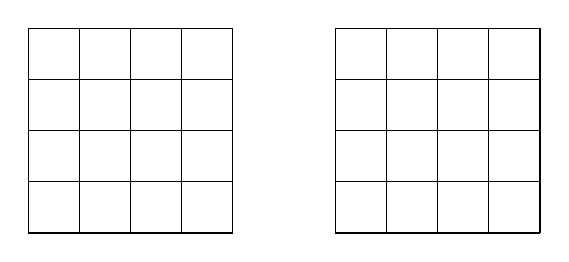
\begin{tikzpicture}[scale=.65]
  \begin{scope}
    \draw (0, 0) grid (4, 4);
    \node at (1.5,3.5) {\symqueen};
    \node at (3.5,2.5) {\symqueen};
    \node at (0.5,1.5) {\symqueen};
    \node at (2.5,0.5) {\symqueen};

    \draw (6, 0) grid (10, 4);
    \node at (6+2.5,3.5) {\symqueen};
    \node at (6+0.5,2.5) {\symqueen};
    \node at (6+3.5,1.5) {\symqueen};
    \node at (6+1.5,0.5) {\symqueen};

  \end{scope}
\end{tikzpicture}
\end{center}

El problema es pot resoldre fent servir backtracking,
col·locant les reines al taulell fila per fila.
Més precisament, per a cada fila, col·locarem una sola reina
i de manera que cap de les reines anteriors l'ataqui.
Quan col·loquem $n$ reines haurem trobat una solució
al problem.

Per exemple, quan $n=4$,
aquestes són algunes solucions parcials generades per
l'algorisme de backtracking:

\begin{center}
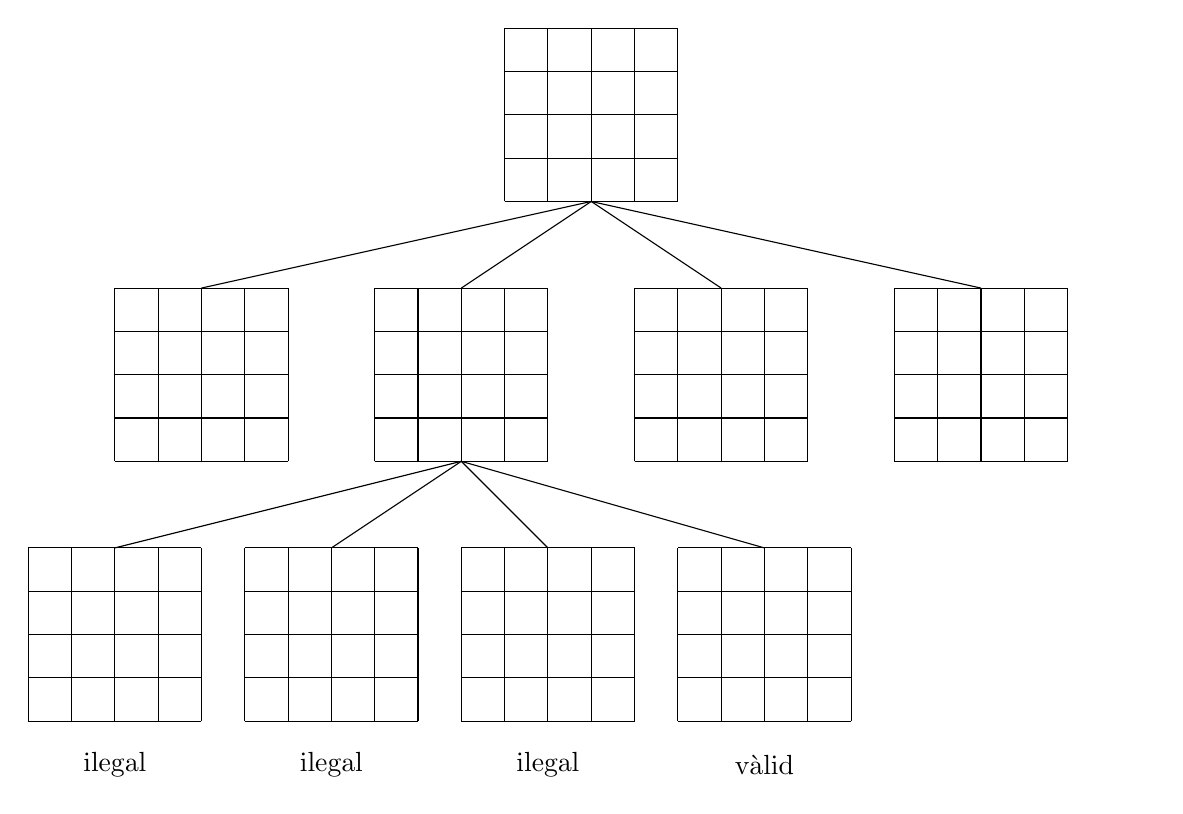
\begin{tikzpicture}[scale=.55]
  \begin{scope}
    \draw (0, 0) grid (4, 4);

    \draw (-9, -6) grid (-5, -2);
    \draw (-3, -6) grid (1, -2);
    \draw (3, -6) grid (7, -2);
    \draw (9, -6) grid (13, -2);

    \node at (-9+0.5,-3+0.5) {\symqueen};
    \node at (-3+1+0.5,-3+0.5) {\symqueen};
    \node at (3+2+0.5,-3+0.5) {\symqueen};
    \node at (9+3+0.5,-3+0.5) {\symqueen};

    \draw (2,0) -- (-7,-2);
    \draw (2,0) -- (-1,-2);
    \draw (2,0) -- (5,-2);
    \draw (2,0) -- (11,-2);

    \draw (-11, -12) grid (-7, -8);
    \draw (-6, -12) grid (-2, -8);
    \draw (-1, -12) grid (3, -8);
    \draw (4, -12) grid (8, -8);
    \draw[white] (11, -12) grid (15, -8);
    \node at (-11+1+0.5,-9+0.5) {\symqueen};
    \node at (-6+1+0.5,-9+0.5) {\symqueen};
    \node at (-1+1+0.5,-9+0.5) {\symqueen};
    \node at (4+1+0.5,-9+0.5) {\symqueen};
    \node at (-11+0+0.5,-10+0.5) {\symqueen};
    \node at (-6+1+0.5,-10+0.5) {\symqueen};
    \node at (-1+2+0.5,-10+0.5) {\symqueen};
    \node at (4+3+0.5,-10+0.5) {\symqueen};

    \draw (-1,-6) -- (-9,-8);
    \draw (-1,-6) -- (-4,-8);
    \draw (-1,-6) -- (1,-8);
    \draw (-1,-6) -- (6,-8);

    \node at (-9,-13) {ilegal};
    \node at (-4,-13) {ilegal};
    \node at (1,-13) {ilegal};
    \node at (6,-13) {vàlid};

  \end{scope}
\end{tikzpicture}
\end{center}

Al nivell inferior, els tres primers taulells són
il·legals, perquè les reines s'ataquen entre elles.
Tanmateix, el quart taulell és vàlid,
i es pot estendre a una solució completa posant dues
reines més al tauler.
Només hi ha una manera de col·locar aquestes dues reines.

L'algorisme es pot implementar de la següent manera:
\begin{lstlisting}
int compte = 0;
vector<bool> columna(n), diag1(2*n), diag2(2*n);
  
void cerca(int y) {
    if (y == n) {
        compte++;
        return;
    }
    for (int x = 0; x < n; x++) {
        if (columna[x] || diag1[x+y] || diag2[x-y+n-1]) continue;
        columna[x] = diag1[x+y] = diag2[x-y+n-1] = 1;
        cerca(y+1);
        columna[x] = diag1[x+y] = diag2[x-y+n-1] = 0;
    }
}
\end{lstlisting}

La cerca comença cridant \texttt{cerca(0)}.
La mida del tauler és $n \times n$,
i el codi calcula el nombre de solucions
a \texttt{compte}.

El codi assumeix que les files i columnes
del tauler estan numerats de 0 a $n-1$.
Quan la funció \texttt{cerca} és
crida amb el paràmetre $y$,
col·loca una dama a la fila $y$
i després es crida recursivament amb el paràmetre $y+1$.
Quan $y=n$ s'ha trobat una solució
i la variable \texttt{compte} s'incrementa en un.

El vector \texttt{columna} porta el compte de les columnes
que tenen una reina,
i els vectors \texttt{diag1} i \texttt{diag2}
porten el compte de les diagonals amb reina.
No està permès afegir una altra reina a una
columna o diagonal que ja en conté una.
Per exemple, les columnes i diagonals de
el tauler $4 \times 4$ es numeren de la manera següent:

\begin{center}
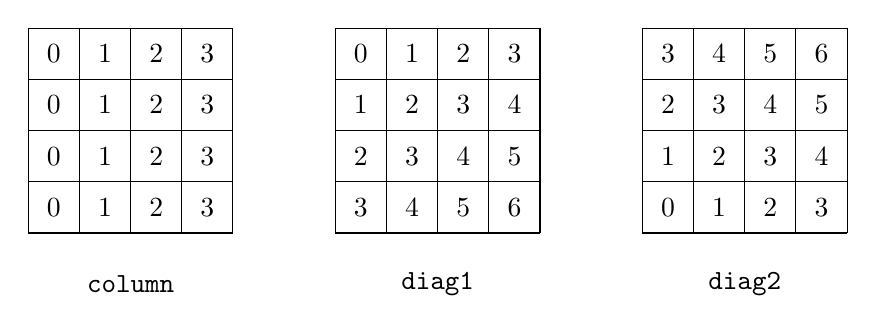
\begin{tikzpicture}[scale=.65]
  \begin{scope}
    \draw (0-6, 0) grid (4-6, 4);
    \node at (-6+0.5,3.5) {$0$};
    \node at (-6+1.5,3.5) {$1$};
    \node at (-6+2.5,3.5) {$2$};
    \node at (-6+3.5,3.5) {$3$};
    \node at (-6+0.5,2.5) {$0$};
    \node at (-6+1.5,2.5) {$1$};
    \node at (-6+2.5,2.5) {$2$};
    \node at (-6+3.5,2.5) {$3$};
    \node at (-6+0.5,1.5) {$0$};
    \node at (-6+1.5,1.5) {$1$};
    \node at (-6+2.5,1.5) {$2$};
    \node at (-6+3.5,1.5) {$3$};
    \node at (-6+0.5,0.5) {$0$};
    \node at (-6+1.5,0.5) {$1$};
    \node at (-6+2.5,0.5) {$2$};
    \node at (-6+3.5,0.5) {$3$};

    \draw (0, 0) grid (4, 4);
    \node at (0.5,3.5) {$0$};
    \node at (1.5,3.5) {$1$};
    \node at (2.5,3.5) {$2$};
    \node at (3.5,3.5) {$3$};
    \node at (0.5,2.5) {$1$};
    \node at (1.5,2.5) {$2$};
    \node at (2.5,2.5) {$3$};
    \node at (3.5,2.5) {$4$};
    \node at (0.5,1.5) {$2$};
    \node at (1.5,1.5) {$3$};
    \node at (2.5,1.5) {$4$};
    \node at (3.5,1.5) {$5$};
    \node at (0.5,0.5) {$3$};
    \node at (1.5,0.5) {$4$};
    \node at (2.5,0.5) {$5$};
    \node at (3.5,0.5) {$6$};

    \draw (6, 0) grid (10, 4);
    \node at (6.5,3.5) {$3$};
    \node at (7.5,3.5) {$4$};
    \node at (8.5,3.5) {$5$};
    \node at (9.5,3.5) {$6$};
    \node at (6.5,2.5) {$2$};
    \node at (7.5,2.5) {$3$};
    \node at (8.5,2.5) {$4$};
    \node at (9.5,2.5) {$5$};
    \node at (6.5,1.5) {$1$};
    \node at (7.5,1.5) {$2$};
    \node at (8.5,1.5) {$3$};
    \node at (9.5,1.5) {$4$};
    \node at (6.5,0.5) {$0$};
    \node at (7.5,0.5) {$1$};
    \node at (8.5,0.5) {$2$};
    \node at (9.5,0.5) {$3$};

    \node at (-4,-1) {\texttt{column}};
    \node at (2,-1) {\texttt{diag1}};
    \node at (8,-1) {\texttt{diag2}};

  \end{scope}
\end{tikzpicture}
\end{center}

Sigui $q(n)$ el nombre de maneres
per posar $n$ reines en un tauler d'escacs $n \times n$.
El procés de backtracking anterior
ens diu que, per exemple, $q(8)=92$.
Quan $n$ augmenta, la cerca es torna lenta ràpidament,
perquè el nombre de solucions augmenta
exponencialment.
Per exemple, calcular $q(16)=14772512$
fent servir l'algorisme anterior triga aproximadament un minut
en un ordinador modern\footnote{No es coneix cap manera de calcular
eficientment valors més grans de $q(n)$. El rècord actual és
$q(27)=234907967154122528$, calculat el 2016 \cite{q27}.}.

\section{Podar la cerca}

Sovint podem optimitzar el backtracking
podant l'arbre de cerca.
La idea és afegir ``intel·ligència'' a l'algorisme
perquè es doni compte com més aviat possible que una
solució parcial no es pot ampliar
a una solució completa.
Aquestes optimitzacions poden tenir un gran impacte
sobre l'eficiència de la cerca.

Considerem el problema
de calcular el nombre de camins
en un taulell $n \times n$ des de la cantonada superior esquerra
a la cantonada inferior dreta de manera que
el camí visiti cada casella exactament una vegada.
Per exemple, en un taulell $7 \times 7$,
hi ha 111712 camins d'aquest tipus.
Un dels camins és el següent:

\begin{center}
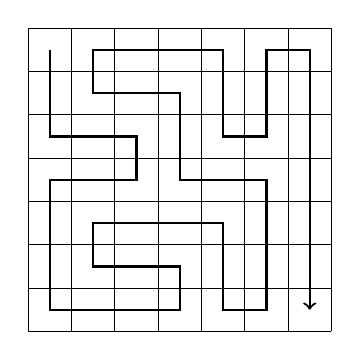
\begin{tikzpicture}[scale=.55]
  \begin{scope}
    \draw (0, 0) grid (7, 7);
    \draw[thick,->] (0.5,6.5) -- (0.5,4.5) -- (2.5,4.5) --
          (2.5,3.5) -- (0.5,3.5) -- (0.5,0.5) --
          (3.5,0.5) -- (3.5,1.5) -- (1.5,1.5) --
          (1.5,2.5) -- (4.5,2.5) -- (4.5,0.5) --
          (5.5,0.5) -- (5.5,3.5) -- (3.5,3.5) --
          (3.5,5.5) -- (1.5,5.5) -- (1.5,6.5) --
          (4.5,6.5) -- (4.5,4.5) -- (5.5,4.5) --
          (5.5,6.5) -- (6.5,6.5) -- (6.5,0.5);
  \end{scope}
\end{tikzpicture}
\end{center}

Ens centrem en el cas de $7 \times 7$,
perquè el seu nivell de dificultat és adequat a les nostres necessitats.
Començarem amb un algorisme de backtracking senzill,
i després l'optimitzarem pas a pas fent servir observacions
de com podem podar la cerca.
Després de cada optimització, mesurarem el temps d'execució
de l'algorisme i el nombre de crides recursives,
per a veure clarament l'efecte de cadascuna d'aquestes
optimitzacions.

\subsubsection{Algorisme bàsic}

La primera versió de l'algorisme no conté
cap optimització. Simplement fem servir el backtracking per generar
tots els camins possibles des de la cantonada superior esquerra fins a
la cantonada inferior dreta i comptar el nombre d'aquests camins.

\begin{itemize}
\item
temps de funcionament: 483 segons
\item
nombre de crides recursives: 76 mil milions
\end{itemize}

\subsubsection{Optimització 1}

En tota solució, primer avancem un pas
cap avall o cap a la dreta.
Sempre hi ha dos camins que
són simètrics
sobre la diagonal del taulell que passa pel primer pas.
Per exemple, els camins següents són simètrics:

\begin{center}
\begin{tabular}{ccc}
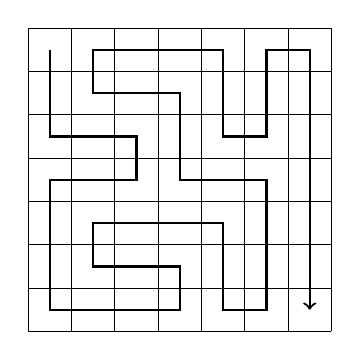
\begin{tikzpicture}[scale=.55]
  \begin{scope}
    \draw (0, 0) grid (7, 7);
    \draw[thick,->] (0.5,6.5) -- (0.5,4.5) -- (2.5,4.5) --
          (2.5,3.5) -- (0.5,3.5) -- (0.5,0.5) --
          (3.5,0.5) -- (3.5,1.5) -- (1.5,1.5) --
          (1.5,2.5) -- (4.5,2.5) -- (4.5,0.5) --
          (5.5,0.5) -- (5.5,3.5) -- (3.5,3.5) --
          (3.5,5.5) -- (1.5,5.5) -- (1.5,6.5) --
          (4.5,6.5) -- (4.5,4.5) -- (5.5,4.5) --
          (5.5,6.5) -- (6.5,6.5) -- (6.5,0.5);
  \end{scope}
\end{tikzpicture}
& \hspace{20px}
& 
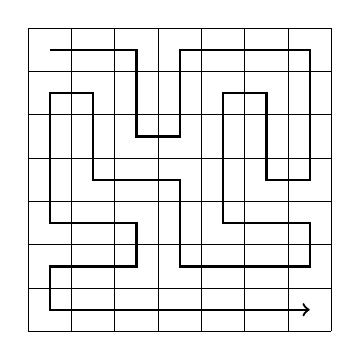
\begin{tikzpicture}[scale=.55]
  \begin{scope}[yscale=1,xscale=-1,rotate=-90]
    \draw (0, 0) grid (7, 7);
    \draw[thick,->] (0.5,6.5) -- (0.5,4.5) -- (2.5,4.5) --
          (2.5,3.5) -- (0.5,3.5) -- (0.5,0.5) --
          (3.5,0.5) -- (3.5,1.5) -- (1.5,1.5) --
          (1.5,2.5) -- (4.5,2.5) -- (4.5,0.5) --
          (5.5,0.5) -- (5.5,3.5) -- (3.5,3.5) --
          (3.5,5.5) -- (1.5,5.5) -- (1.5,6.5) --
          (4.5,6.5) -- (4.5,4.5) -- (5.5,4.5) --
          (5.5,6.5) -- (6.5,6.5) -- (6.5,0.5);
  \end{scope}
\end{tikzpicture}
\end{tabular}
\end{center}

Per tant, podem decidir que el primer pas és sempre cap avall
(o cap a la dreta),
i multiplicar per dos el nombre de solucions.

\begin{itemize}
\item
temps de funcionament: 244 segons
\item
nombre de crides recursives: 38 mil milions
\end{itemize}

\subsubsection{Optimització 2}

Si el camí arriba al quadrat inferior dret
abans d'haver visitat tots els altres quadrats de la quadrícula,
està clar que no serà possible completar la solució.
Un exemple d'això és el camí següent:

\begin{center}
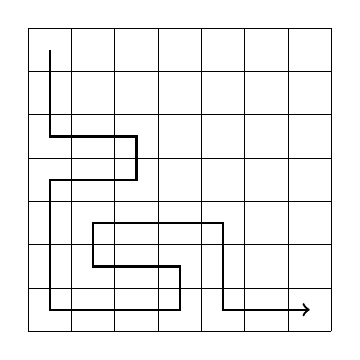
\begin{tikzpicture}[scale=.55]
  \begin{scope}
    \draw (0, 0) grid (7, 7);
    \draw[thick,->] (0.5,6.5) -- (0.5,4.5) -- (2.5,4.5) --
          (2.5,3.5) -- (0.5,3.5) -- (0.5,0.5) --
          (3.5,0.5) -- (3.5,1.5) -- (1.5,1.5) --
          (1.5,2.5) -- (4.5,2.5) -- (4.5,0.5) --
          (6.5,0.5);
  \end{scope}
\end{tikzpicture}
\end{center}
Amb aquesta observació, podem acabar la cerca
immediatament si arribem massa aviat a la casella inferior dreta.
\begin{itemize}
\item
temps de funcionament: 119 segons
\item
nombre de crides recursives: 20 mil milions
\end{itemize}

\subsubsection{Optimització 3}

Si el camí toca una paret
i pot girar a l'esquerra o a la dreta,
la graella es divideix en dues parts
que contenen caselles no visitades.
Per exemple, en la situació següent,
el camí pot girar a l'esquerra o a la dreta:

\begin{center}
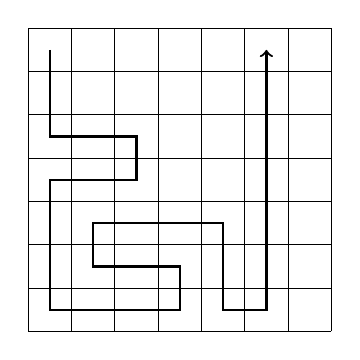
\begin{tikzpicture}[scale=.55]
  \begin{scope}
    \draw (0, 0) grid (7, 7);
    \draw[thick,->] (0.5,6.5) -- (0.5,4.5) -- (2.5,4.5) --
          (2.5,3.5) -- (0.5,3.5) -- (0.5,0.5) --
          (3.5,0.5) -- (3.5,1.5) -- (1.5,1.5) --
          (1.5,2.5) -- (4.5,2.5) -- (4.5,0.5) --
          (5.5,0.5) -- (5.5,6.5);
  \end{scope}
\end{tikzpicture}
\end{center}
En aquest cas, ja no podem visitar totes les caselles,
i podem acabar la cerca. Aquesta optimització és molt útil:

\begin{itemize}
\item
temps de funcionament: $1.8$ segons
\item
nombre de crides recursives: 221 milions
\end{itemize}

\subsubsection{Optimització 4}

La idea de l'optimització 3
es pot generalitzar:
si el camí no pot continuar endavant
però pot girar a l'esquerra o a la dreta,
el taulell es divideix en dues parts
que contenen caselles no visitades.
Per exemple, considerem el camí següent:

\begin{center}
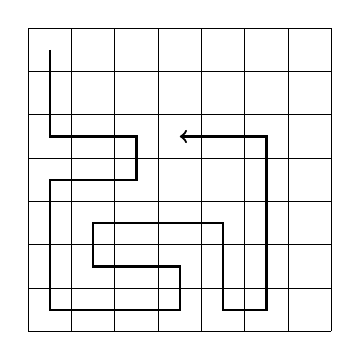
\begin{tikzpicture}[scale=.55]
  \begin{scope}
    \draw (0, 0) grid (7, 7);
    \draw[thick,->] (0.5,6.5) -- (0.5,4.5) -- (2.5,4.5) --
          (2.5,3.5) -- (0.5,3.5) -- (0.5,0.5) --
          (3.5,0.5) -- (3.5,1.5) -- (1.5,1.5) --
          (1.5,2.5) -- (4.5,2.5) -- (4.5,0.5) --
          (5.5,0.5) -- (5.5,4.5) -- (3.5,4.5);
  \end{scope}
\end{tikzpicture}
\end{center}
Està clar que ja no podem visitar totes les caselles,
de manera que acabem la cerca. Després d'aquesta optimització,
la cerca és molt eficient:

\begin{itemize}
\item
temps de funcionament: $0.6$ segons
\item
nombre de crides recursives: 69 milions
\end{itemize}

~\\
Ara és un bon moment per deixar d'optimitzar
l'algorisme i veure què hem aconseguit.
El temps d'execució de l'algorisme original
era 483 segons i, després de les optimitzacions,
el temps ha baixat a només $0.6$ segons.
Les optimitzacions han fet que l'algorisme sigui
gairebé 1000 vegades més ràpid.

Aquest és un fenomen habitual en el backtracking,
perquè els arbres de cerca solen ser molt grans
i fins i tot observacions simples poden podar eficaçment
la cerca.
Les optimitzacions que es produeixen durant els primers
passos de l'algorisme, és a dir, a la part superior de
l'arbre de cerca, són especialment útils.

\section{Trobar-se al mig}

\index{trobar-se al mig}

\key{Trobar-se al mig} és una tècnica
on es divideix l'espai de cerca
en dues parts d'aproximadament la mateixa mida.
Es realitzen cerques independents
per a cada part,
i finalment es combinen els resultats de les cerques.

La tècnica es pot fer servir
si hi ha una manera eficient de combinar el
resultats de les cerques.
En aquesta situació, les dues cerques poden requerir menys
temps que una cerca gran.
Típicament, fent servir la tècnica de trobar-se al mig podem
transformar un factor $2^n$ en un factor $2^{n/2}$.

Com a exemple, considerem el problema on
se'ns dóna una llista de $n$ nombres i
un nombre $x$,
i volem saber si és possible
triar alguns números de la llista de manera que
la seva suma sigui $x$.
Per exemple, donada la llista $[2,4,5,9]$ i $x=15$,
podem triar els números $[2,4,9]$ per obtenir $2+4+9=15$.
Tanmateix, fent servir la mateixa llista i $x=10$, ja no
és possible obtenir la suma.

Un algorisme senzill que resol el problema és
iterar tots els subconjunts dels elements i
comprovar si la suma d'algun dels subconjunts és $x$.
El temps d'execució d'aquest algorisme és $O(2^n)$,
perquè hi ha $2^n$ subconjunts.
No obstant això, fent servir la tècnica de trobar-se al mig,
podem aconseguir un algorisme de temps $O(2^{n/2})$ més eficient\footnote{Aquesta idea va ser introduïda l'any 1974 per E. Horowitz
i S. Sahni \cite{hor74}.}.
Tingueu en compte que $O(2^n)$ i $O(2^{n/2})$ són diferents
complexitats perquè $2^{n/2}$ és igual a $\sqrt{2^n}$.

La idea és dividir la llista en
dues llistes $A$ i $B$ de manera que cada llista
contingui aproximadament la meitat dels números.
La primera cerca genera tots els subconjunts
de $A$ i emmagatzema les seves sumes en una llista $S_A$.
De manera semblant, la segona cerca
crea una llista $S_B$ a partir de $B$.
Després d'això, n'hi ha prou comprovant si és possible
triar un element de $S_A$ i un altre
de $S_B$ de manera que la seva suma sigui $x$.
Això només és possible si hi ha alguna manera de formar la suma
$x$ amb els números de la llista original.

Per exemple, suposem que la llista és $[2,4,5,9]$ i $x=15$.
Primer, dividim la llista en $A=[2,4]$ i $B=[5,9]$.
Després d'això, creem llistes
$S_A=[0,2,4,6]$ i $S_B=[0,5,9,14]$.
En aquest cas, podem formar la suma $x=15$,
perquè $S_A$ conté la suma $6$,
$S_B$ conté la suma $9$ i $6+9=15$.
Això correspon a la solució $[2,4,9]$.

Podem implementar l'algorisme de manera que
la seva complexitat temporal és $O(2^{n/2})$.
Primer, generem llistes \emph{ordenades} $S_A$ i $S_B$,
que es pot fer en $O(2^{n/2})$, fent servir una tècnica semblant
a la fusió (\texttt{merge}). Després, donat que les llistes estan
ordenades, podem comprovat en temps $O(2^{n/2})$ si
la suma $x$ es pot crear a partir de $S_A$ i $S_B$.
